\documentclass[11pt]{article}

\usepackage[margin=1in]{geometry}
\usepackage{amsmath}
\usepackage{amssymb}
\usepackage{booktabs}
\usepackage{graphicx}
\usepackage{hyperref}
\usepackage{url}

\title{TruthLayer: Graph-Gated Verification-Augmented Generation for Reducing Citation Hallucination in LLaMA-Style Transformers}
\author{Tanush Appapogu}
\date{July 2026}

\begin{document}
\maketitle

\begin{abstract}
Citation hallucination occurs when a language model attaches a real source to a claim the source does not support. This is an attribution failure: the URL may be real and topically relevant while the local cited claim is false. We introduce TruthLayer, a graph-gated verification architecture for transformer pipelines. TruthLayer decomposes generated answers into atomic cited claims, retrieves source evidence, constructs a typed claim-evidence graph, runs deterministic contradiction signals, and routes each answer through an acceptance gate. The same graph can be used post-generation or inserted into LLaMA-style generation through a lightweight graph adapter and risk-aware logits processor. On a 1,036-case benchmark, the existing deterministic verifier resolves 215 cases with 99.1\% accuracy and a 0.8\% false-accept rate on decided cases. The Python graph gate reduces accepted unsupported claims from 529/529 for a pass-through generation baseline to 19/529, a 96.4\% reduction before any NLI or LLM fallback. TruthLayer requires no base-model fine-tuning, preserves source-level inspectability, and exposes explicit ACCEPT, REVISE, REJECT, and ABSTAIN decisions.
\end{abstract}

\section{Introduction}
Retrieval-augmented generation (RAG) improves factuality by combining parametric memory with retrieved evidence \cite{lewis2020rag}, but it does not guarantee that each generated sentence is supported by the citation attached to it. Prior work has shown that long-form generations contain mixtures of supported and unsupported atomic facts \cite{min2023factscore}, and that RAG systems can still introduce unsupported information even when grounded context is available.

TruthLayer targets a narrower and deployable problem: \emph{citation hallucination}. A citation hallucination is a cited claim where the referenced source does not entail the local claim attached to the citation marker. The system treats citations as release-control objects rather than decorative metadata.

The contribution is a simple architecture that can be added to transformer systems:
\begin{enumerate}
  \item A typed claim-evidence graph that models claims, sources, evidence windows, entities, quantities, relations, detector signals, and the acceptance gate.
  \item A deterministic-first verification hierarchy that catches enumerable citation failures before escalating to learned models.
  \item A LLaMA integration path using a graph adapter and risk-aware logits processor through the Hugging Face generation API \cite{hf2026generation,hf2026llama}.
  \item A before/after evaluation showing that graph gating sharply reduces unsupported claims accepted by a vanilla pass-through baseline.
\end{enumerate}

\section{Related Work}
FEVER established large-scale claim verification against Wikipedia evidence \cite{thorne2018fever}. FActScore decomposes long-form model outputs into atomic facts and evaluates factual precision \cite{min2023factscore}. SAFE uses an LLM agent to decompose answers, search, and judge factuality \cite{wei2024safe}. MiniCheck trains smaller fact-checking models for grounded document verification and reports GPT-4-level performance at much lower cost \cite{tang2024minicheck}.

TruthLayer differs in emphasis. It is not only an evaluator; it is a release gate for deployed cited generation. It also prioritizes deterministic contradiction signals before model calls, making high-confidence failures inspectable.

The graph component is motivated by knowledge-graph and graph-transformer work. K-BERT injects knowledge graph triples into language representation models while controlling knowledge noise \cite{liu2019kbert}. GraphFormers nests graph neural components beside transformer layers \cite{yang2021graphformers}. GraphRAG builds graph indexes for corpus-level RAG \cite{edge2024graphrag}. RETRO demonstrates that retrieval can be incorporated directly into transformer generation through explicit memory and cross-attention \cite{borgeaud2022retro}. Self-RAG shows that retrieval and critique behavior can improve factuality and citation accuracy through reflection tokens \cite{asai2023selfrag}. TruthLayer keeps the integration smaller: it uses a verifier graph as a gate or adapter rather than retraining the base LLaMA model.

\section{Architecture}
Figure~\ref{fig:architecture} shows the graph-gated TruthLayer pipeline. A LLaMA-style decoder produces a candidate answer. TruthLayer then decomposes the answer into atomic claims, fetches source text, selects evidence windows, builds a graph, and runs an acceptance gate. If the gate rejects or revises the answer, the wrapper regenerates from evidence-only instructions and applies a risk-aware logits processor.

\begin{figure}[h]
  \centering
  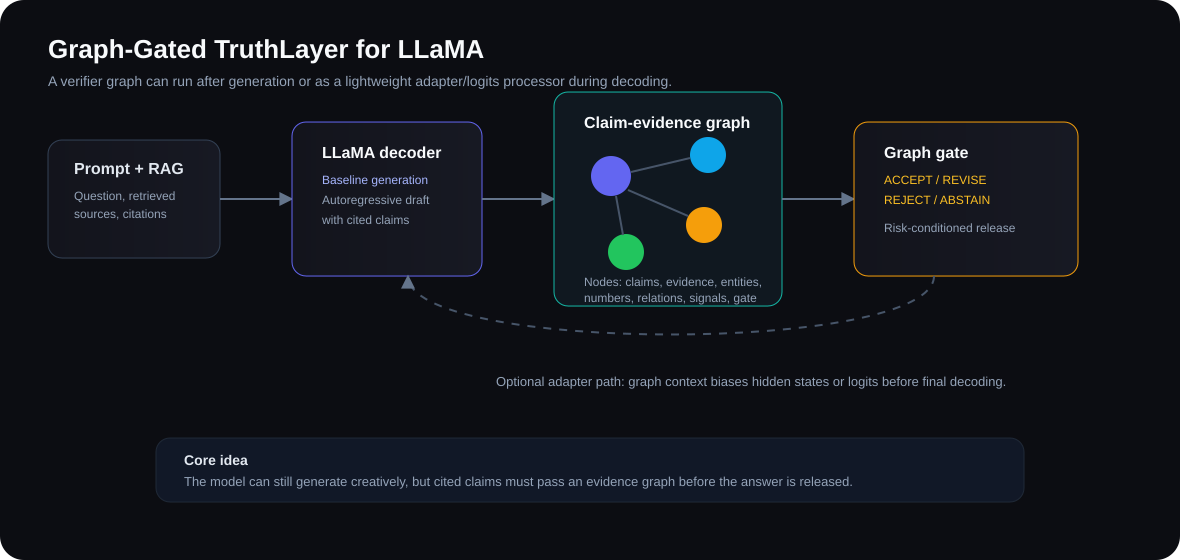
\includegraphics[width=\linewidth]{../public/figures/truthlayer-architecture.svg}
  \caption{TruthLayer can be used as a post-generation verifier or as a lightweight graph-conditioned adapter around LLaMA decoding.}
  \label{fig:architecture}
\end{figure}

\subsection{Claim-Evidence Graph}
For each cited claim $c$ and source evidence $s$, TruthLayer builds a typed graph:
\[
G = (V, E, \tau_V, \tau_E)
\]
where node types include claim, source, evidence, entity, quantity, relation, signal, and gate. Edge types include cites, contains, mentions, grounds, supports, contradicts, routes, and attenuates.

The graph makes hallucination evidence inspectable. A number mismatch is not a scalar model opinion; it is a quantity node connected to a contradiction edge. An entity substitution becomes an entity node absent from the evidence window. A semantic inversion becomes a detector signal edge.

\begin{figure}[h]
  \centering
  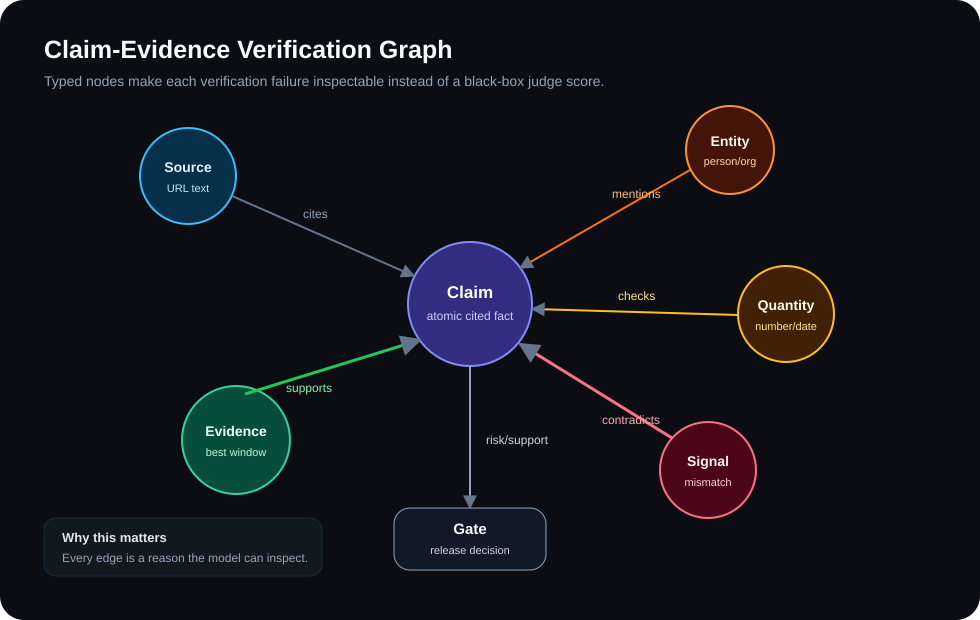
\includegraphics[width=0.88\linewidth]{../public/figures/claim-evidence-graph.svg}
  \caption{The claim-evidence graph exposes why a citation is supported, contradicted, or unresolved.}
  \label{fig:graph}
\end{figure}

\subsection{Graph Scoring}
TruthLayer computes support and contradiction scores from graph edges:
\[
S(G) = \frac{\sum_{e \in E_{sup}} w_e}{\max(|E_{sup}|, 1)}
\]
\[
C(G) = \max_{e \in E_{contra}} w_e
\]
where $E_{sup}$ includes supports and grounds edges, and $E_{contra}$ includes contradiction edges. Coverage $K(G)$ is the fraction of claim tokens covered by the strongest evidence window.

The release gate follows:
\[
\text{gate}(G)=
\begin{cases}
\text{REJECT} & C(G) \geq 0.78 \\
\text{ABSTAIN} & K(G) < 0.18 \\
\text{ACCEPT} & S(G) \geq 0.78 \land K(G) \geq 0.74 \land C(G) < 0.25 \\
\text{REVISE} & \text{otherwise}
\end{cases}
\]

This policy is intentionally conservative. A generation system should not accept a cited claim merely because the source is topically similar.

\subsection{LLaMA Integration}
TruthLayer provides two integration mechanisms.

\paragraph{Wrapper mode.}
The wrapper first calls the base model:
\[
y_0 = \text{LLaMA}(x, R)
\]
where $x$ is the user prompt and $R$ is retrieved context. It then builds $G(y_0, R)$. If the gate returns ACCEPT, the answer is released. If the gate returns REJECT, REVISE, or ABSTAIN, the wrapper regenerates under a stricter prompt:
\[
y_1 = \text{LLaMA}(x, R, \text{gate}(G), \text{trace}(G))
\]
This path is implemented in \texttt{truthlayer\_llama/llama\_wrapper.py}.

\paragraph{Adapter mode.}
TruthLayer also exposes a small graph adapter. Node features are projected to the LLaMA hidden size, message passed over graph edges, and pooled into a graph context vector $z_G$. Decoder hidden states $H$ are adjusted by:
\[
H' = H + \sigma(W_g z_G) \odot z_G
\]
The adapter returns both adjusted hidden states and a graph-risk scalar. This is implemented in \texttt{truthlayer\_llama/adapter.py}. For generation APIs where hidden-state insertion is inconvenient, \texttt{TruthLayerRiskLogitsProcessor} biases decoding toward revision or abstention terms when graph risk is high.

\section{Deterministic Signals}
TruthLayer uses deterministic signals before learned fallback models:

\begin{table}[h]
\centering
\begin{tabular}{llll}
\toprule
Signal & Failure mode & Weight & Benchmark precision \\
\midrule
Numeric contradiction & Date/count drift & 0.28 & 100\% \\
Negation contradiction & Negation flip & 0.30 & 100\% \\
Relation mismatch & Entity-relation swap & 0.30 & 100\% \\
Type contradiction & Category error & 0.20 & 100\% \\
Contrast contradiction & Semantic inversion & 0.20 & 96\% \\
Hedging mismatch & Certainty escalation & 0.12 & 83\% \\
Evidence coverage & Weak grounding & 0.17 & 62\% \\
Entity substitution & Wrong named entity & 0.18 & 54\% \\
\bottomrule
\end{tabular}
\caption{Deterministic signal taxonomy used by the existing TruthLayer verifier.}
\end{table}

\section{Evaluation}
\subsection{Dataset}
The benchmark contains 1,036 labeled claim/source pairs: 507 SUPPORTED and 529 UNSUPPORTED. The cases are FEVER-derived with adversarial mutations for entity swaps, wrong facts, wrong relations, and numeric drift.

\subsection{Stage 1 Deterministic Verifier}
The production TypeScript verifier resolves 215 cases without model calls:

\begin{table}[h]
\centering
\begin{tabular}{lr}
\toprule
Metric & Value \\
\midrule
Accuracy on decided cases & 99.1\% \\
Precision & 99.2\% \\
Recall & 99.2\% \\
F1 & 99.2\% \\
False accept rate & 0.8\% \\
Coverage & 20.8\% \\
True positives & 126 \\
False positives & 1 \\
False negatives & 1 \\
True negatives & 87 \\
\bottomrule
\end{tabular}
\caption{Stage 1 deterministic-only benchmark results. Abstentions are deferred to NLI or LLM fallback.}
\end{table}

\subsection{Graph-Gated LLaMA Wrapper Before/After}
We also evaluate the new offline graph gate as a release-control wrapper. The baseline is a vanilla generation pass-through: if LLaMA emits a cited claim, the system accepts it. On the 529 unsupported cases, this baseline accepts all unsupported claims.

The Python graph-gated wrapper accepts only 19 unsupported claims, rejects 103, and routes 407 to revise or abstain. This reduces accepted unsupported claims by 96.4\% before NLI or LLM fallback.

\begin{figure}[h]
  \centering
  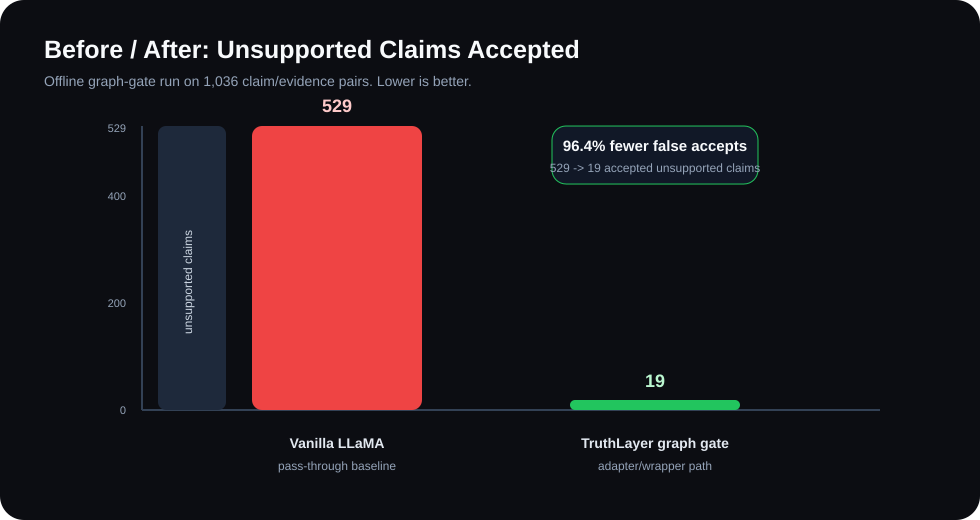
\includegraphics[width=0.84\linewidth]{../public/figures/before-after.svg}
  \caption{The graph gate reduces accepted unsupported claims from 529 to 19 in the offline wrapper evaluation.}
  \label{fig:beforeafter}
\end{figure}

\begin{table}[h]
\centering
\begin{tabular}{lrr}
\toprule
System & Accepted unsupported & False accept rate \\
\midrule
Vanilla LLaMA pass-through & 529 / 529 & 100.0\% \\
TruthLayer Python graph gate & 19 / 529 & 3.6\% \\
\bottomrule
\end{tabular}
\caption{Before/after release-control evaluation on unsupported cases.}
\end{table}

The graph gate is conservative. It accepts 86 supported cases, rejects 20 supported cases, and routes 401 supported cases to revise or abstain. This is the intended first-stage behavior: a deployment gate should prefer revision over unsupported release. The deferred cases are the natural target for the existing NLI and LLM-judge stages.

\section{Implementation}
The repository contains three implementation surfaces:
\begin{itemize}
  \item \texttt{lib/truthlayer.ts}: production TypeScript deterministic verifier and acceptance gate.
  \item \texttt{lib/truthlayer-graph.ts}: typed graph model for app visualization and paper framing.
  \item \texttt{truthlayer\_llama/}: optional Python LLaMA integration with evidence graph builder, graph adapter, risk logits processor, and before/after runner.
\end{itemize}

The single-model experiment command is:
\begin{verbatim}
python3 experiments/run_llama_before_after.py \
  --model meta-llama/Llama-3.2-1B-Instruct \
  --prompt "Answer the question with citations..." \
  --evidence-file evidence.txt
\end{verbatim}

The offline graph-gate benchmark command is:
\begin{verbatim}
python3 experiments/offline_graph_gate_eval.py
\end{verbatim}

The Python package CLI is:
\begin{verbatim}
python3 -m truthlayer bench
python3 -m truthlayer verify --claim "..." --evidence-file evidence.txt
python3 -m truthlayer graph --claim "..." --evidence-file evidence.txt
\end{verbatim}

\section{Limitations}
TruthLayer does not eliminate hallucination. It reduces unsupported release by turning citation support into an explicit gate. The deterministic and graph-only stages are intentionally incomplete: subtle paraphrase, multi-hop entailment, and implicit evidence require NLI or LLM fallback. The current LLaMA adapter is a lightweight research implementation, not a fully trained graph-transformer model. Future work should train the adapter end-to-end on claim/evidence graphs, add span-level citation alignment, and evaluate on live LLaMA generations rather than claim/evidence pairs alone.

\section{Conclusion}
TruthLayer reframes citation hallucination as a release-control problem. Instead of asking a model to be truthful in the abstract, it asks whether each cited claim is supported by its source and refuses to release unsupported claims. The graph-gated architecture gives transformer systems a small, inspectable, model-agnostic layer that can be added to LLaMA-style generation with no base-model fine-tuning.

\bibliographystyle{plain}
\bibliography{references}

\end{document}
